%Este trabalho está licenciado sob a Licença Atribuição-CompartilhaIgual 4.0 Internacional Creative Commons. Para visualizar uma cópia desta licença, visite http://creativecommons.org/licenses/by-sa/4.0/deed.pt_BR ou mande uma carta para Creative Commons, PO Box 1866, Mountain View, CA 94042, USA.

\chapter{Cônicas}\label{cap_conicas}
\thispagestyle{fancy}

Neste capítulo, fazemos um estudo introdutório sobre cônicas no plano cartesiano. Mais precisamente, vamos estudar as equações de elipses, hipérboles e parábolas.

\section{Elipse}\label{cap_conicas_sec_elipse}

Sejam $F_1$, $F_2$ pontos sobre um plano $\pi$, $c = \frac{1}{2}|F_1F_2|$ e $a > c$. Chama-se \emph{elipse} de \emph{focos} $F_1$ e $F_2$ ao conjunto de pontos $P$ tais que
\begin{equation}
  {\color{blue}|PF_1| + |PF_2| = 2a}.
\end{equation}
Veja a Figura \ref{fig:elipse}.

\begin{figure}[H]
  \centering
  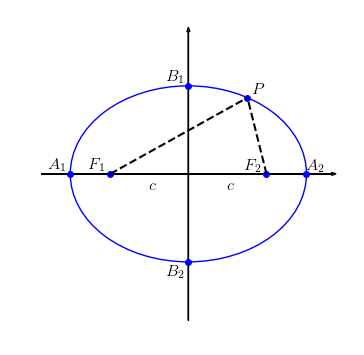
\includegraphics[width=0.7\textwidth]{./cap_conicas/dados/fig_elipse/fig_elipse}
  \caption{Ilustração de uma elipse de focos $F_1$ e $F_2$.}
  \label{fig:elipse}
\end{figure}

Dada uma tal elipse, identificamos $2c=|F_1F_2|$ como a \emph{distância focal}. Os pontos $A_1$ e $A_2$ de interseção da elipse com a reta que passa pelos focos são chamados de \emph{vértices} da elipse. O segmento $A_1A_2$ é chamado de \emph{eixo maior} da elipse. Observamos que
\begin{equation}
  |A_1A_2| = 2a.
\end{equation}
O ponto médio do segmento $F_1F_2$ é chamado de \emph{centro} da elipse. Sejam $B_1$ e $B_2$ os pontos de interseção da elipse com a reta que passa pelo centro da elipse e é perpendicular ao segmento $A_1A_2$. Assim sendo, o segmento $B_1B_2$ é chamado de \emph{eixo menor} da elipse. Vamos denotar
\begin{equation}
  2b = |B_1B_2|.
\end{equation}

Chamamos de \emph{excentricidade} da elipse o número
\begin{equation}
  e = \frac{c}{a}.
\end{equation}
Notemos que $0 \leq e < 1$. Para $e=0$, temos $c=0$ e, portanto $F_1=F_2$. Neste caso, a elipse é a circunferência de centro em $F_1$ (ou $F_2$) e diâmetro $2a$. No que $e$ tende a $1$, a elipse tende ao segmento $A_1A_2$.

Por fim, notamos que o triângulo $B_1OF_2$ é retângulo, $|OF_2|=c$, $|F_2B_1|=a$ e $|OB_1|=b$. Do teorema de Pitágoras segue
\begin{equation}\label{eq:elipse_obs}
  b^2 + c^2 = a^2.
\end{equation}

\subsection{Equação reduzida da elipse}

Consideremos o sistema de coordenadas cartesianas. Sejam $F_1=(-c,0)$ e $F_2=(c,0)$, $c\geq 0$, os focos de uma dada elipse (veja a Figura \ref{fig:elipse}).  Se $P=(x,y)$ é um ponto da elipse, então
\begin{equation}
  |PF_1| + |PF_2| = 2a.
\end{equation}
Como
\begin{align}
  |PF_1| &= \sqrt{(x+c)^2 + y^2}, \\
  |PF_2| &= \sqrt{(x-c)^2 + y^2},
\end{align}
temos
\begin{equation}
  \sqrt{(x+c)^2 + y^2} + \sqrt{(x-c)^2 + y^2} = 2a,
\end{equation}
ou, equivalentemente,
\begin{equation}
  \sqrt{(x+c)^2 + y^2} = 2a - \sqrt{(x-c)^2 + y^2}.
\end{equation}
Elevando ao quadrado, obtemos
\begin{equation}
  (x+c)^2 + y^2 = 4a^2 - 4a\sqrt{(x-c)^2+y^2} + (x-c)^2+y^2.
\end{equation}
Por cancelamento e rearranjo dos termos, obtemos
\begin{equation}
  a\sqrt{(x-c)^2+y^2}=a^2-cx.
\end{equation}
Elevando novamente ao quadrado, temos
\begin{equation}
  a^2(x-c)^2+a^2y^2=a^4-2a^2cx+c^2x^2,
\end{equation}
donde
\begin{equation}
  a^2x^2 -2a^2cx + a^2c^2 + a^2y^2= a^4 -2a^2cx + c^2x^2.
\end{equation}
Por cancelamento e rearranjo dos termos, obtemos
\begin{equation}
  x^2(a^2 - c^2) + a^2y^2 = a^2(a^2 - c^2).
\end{equation}
Como $a>c$, dividimos por $a^2-c^2$  e depois por $a^2$ para obtemos
\begin{equation}
  \frac{x^2}{a^2} + \frac{y^2}{a^2-c^2} = 1.
\end{equation}
Por fim, da equação \eqref{eq:elipse_obs}, temos $a^2-c^2 = b^2$, o que nos leva  a \emph{equação reduzida da elipse}
\begin{equation}
  {\color{blue}\frac{x^2}{a^2} + \frac{y^2}{b^2} = 1}.
\end{equation}

\begin{ex}
  A Figura \ref{fig:elipse_ex} é um esboço do gráfico da elipse de equação reduzida
  \begin{equation}
    \frac{x^2}{25} + \frac{y^2}{16} = 1.
  \end{equation}

  \begin{figure}[H]
    \centering
    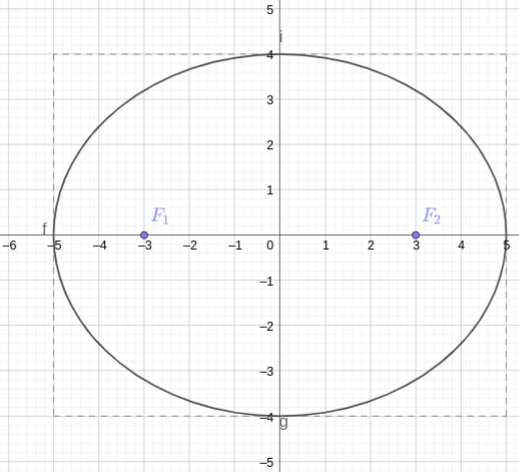
\includegraphics[width=0.5\textwidth]{cap_conicas/dados/fig_ex_elipse/fig}
    \caption{Esboço do gráfico da elipse $\displaystyle\frac{x^2}{25}-\frac{y^2}{16}=1$.}
    \label{fig:elipse_ex}
  \end{figure}
\end{ex}

\subsection*{Exercícios resolvidos}

\begin{exeresol}
  Determine a equação reduzida da elipse de focos $F_1=(-3,0)$, $F_2=(3,0)$ e vértices $A_1=(-5,0)$ e $A_2=(5,0)$.
\end{exeresol}
\begin{resol}
  A equação reduzida tem a forma
  \begin{equation}
    \frac{x^2}{a^2} + \frac{y^2}{b^2} = 1,
  \end{equation}
  onde
  \begin{equation}
    b^2 + c^2 = a^2.
  \end{equation}
  Dos focos temos $c=3$ e dos vértices temos $a=5$. Logo,
  \begin{align}
    b^2 &=  a^2 - c^2 \\
        &= 5^2 - 3^2 \\
        &= 25 - 9 \\
        &= 16.
  \end{align}
  Concluímos que a elipse em questão tem equação
  \begin{equation}
    \frac{x^2}{25} - \frac{y^2}{16} = 1.
  \end{equation}
\end{resol}

\begin{exeresol}
  Determine os focos da elipse de equação
  \begin{equation}
    \frac{x^2}{16} + \frac{y^2}{25} = 1.
  \end{equation}
\end{exeresol}
\begin{resol}
  Começamos lembrando que os focos de uma elipse estão localizados sobre seu eixo maior. No caso deste exercício, temos $a=4$ e $b=5$, logo o eixo maior é $B_1B_2$, na mesma direção do eixo das ordenadas $Oy$. Do triângulo retângulo $OA_2F_1$ temos
  \begin{equation}
    b^2 = a^2 + c^2,
  \end{equation}
  veja a Figura \ref{fig:elipse_exeresol1}.

  \begin{figure}[H]
    \centering
    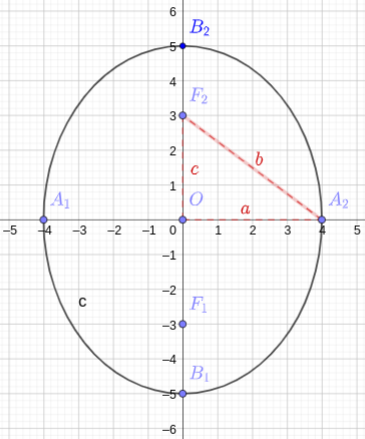
\includegraphics[width=0.5\textwidth]{cap_conicas/dados/fig_elipse_exeresol1/fig}
    \caption{Esboço do gráfico de uma elipse com eixo maior sobre o eixo das ordenadas $Oy$.}
    \label{fig:elipse_exeresol1}
  \end{figure}

  Daí, temos
  \begin{align}
    c^2 &= b^2 - a^2 \\
        &= 25 - 16 \\
        &= 9 \\
    c &= 3.
  \end{align}
  Concluímos que os focos são $F_1=(0,-3)$ e $F_2=(0,3)$.
\end{resol}

\subsection*{Exercícios}

\begin{exer}
  Faça um esboço da elipse de equação reduzida
  \begin{equation}
    \frac{x^2}{9} + \frac{y^2}{4} = 1.
  \end{equation}
\end{exer}
\begin{resp}
  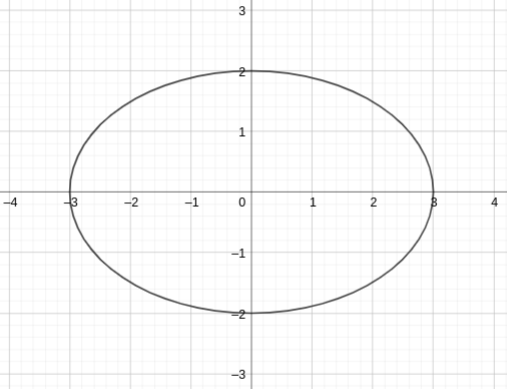
\includegraphics[width=0.5\textwidth]{cap_conicas/dados/fig_elipse_exer_ox/fig}
\end{resp}

\begin{exer}
  Faça um esboço da elipse de equação reduzida
  \begin{equation}
    \frac{x^2}{4} + \frac{y^2}{9} = 1.
  \end{equation}
\end{exer}
\begin{resp}
  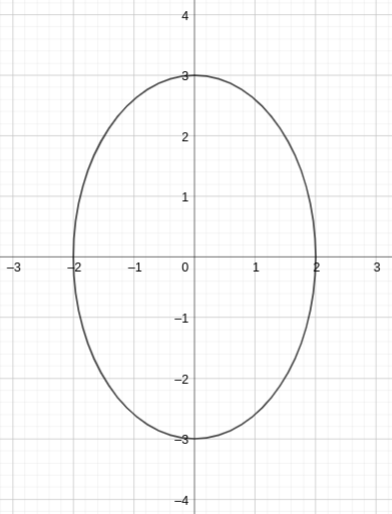
\includegraphics[width=0.4\textwidth]{cap_conicas/dados/fig_elipse_exer_oy/fig}
\end{resp}

\begin{exer}
  Determine os vértices (sobre o eixo maior) das seguintes elipses:
  \begin{enumerate}[a)]
  \item $\displaystyle \frac{x^2}{9} + \frac{y^2}{4} = 1$
  \item $\displaystyle x^2 + \frac{y^2}{16} = 1$
  \end{enumerate}
\end{exer}
\begin{resp}
  a)~$(-3, 0)$, $(3, 0)$; b)~$(0, -4)$, $(0, 4)$
\end{resp}

\begin{exer}
  Determine os focos das seguintes elipses:
  \begin{enumerate}[a)]
  \item $\displaystyle \frac{x^2}{9} + \frac{y^2}{4} = 1$
  \item $\displaystyle x^2 + \frac{y^2}{16} = 1$
  \end{enumerate}
\end{exer}
\begin{resp}
  a)~$(-\sqrt{5}, 0)$, $(\sqrt{5}, 0)$; b)~$(0, \sqrt{15})$, $(0, \sqrt{15})$
\end{resp}

\begin{exer}
  Forneça a equação reduzida da elipse de focos $F_1=(-1, 0)$, $F_2=(1, 0)$ e vértices $A_1=(-\sqrt{2}, 0)$, $A_2=(\sqrt{2}, 0)$.
\end{exer}
\begin{resp}
  $\displaystyle\frac{x^2}{2}+y^2=1$
\end{resp}

\begin{exer}
  Forneça a equação reduzida da elipse de focos $F_1=(0, -2)$, $F_2=(0, 2)$ e vértices $B_1=(0, -\sqrt{5})$, $B_2=(0, \sqrt{5})$.
\end{exer}
\begin{resp}
  $\displaystyle x^2+\frac{y^2}{5}=1$
\end{resp}

\section{Hipérbole}\label{cap_conicas_sec_hiperbole}

Sejam $F_1$ e $F_2$ pontos sobre um plano $\pi$. Sejam, também, $c$ tal que $|F_1F_2|=2c$ e $a<c$. O lugar geométrico dos pontos $P$ tais que
\begin{equation}
  {\color{blue}||PF_1|-|PF_2||=2a},
\end{equation}
chama-se \emph{hipérbole}. Veja Figura \ref{fig:hiperbole}.

\begin{figure}[H]
  \centering
  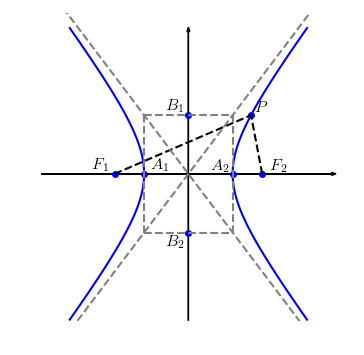
\includegraphics[width=0.7\textwidth]{./cap_conicas/dados/fig_hiperbole/fig_hiperbole}
  \caption{Ilustração de uma hipérbole de focos $F_1$ e $F_2$.}
  \label{fig:hiperbole}
\end{figure}

Os pontos $F_1$ e $F_2$ são chamados de \emph{focos} da hipérbole e $2c = |F_1F_2|$ é chamada de \emph{distância focal}. O ponto médio entre os pontos $F_1$ e $F_2$ é chamado de centro da hipérbole. São chamados \emph{vértices} da hipérbole os pontos $A_1$ e $A_2$, sendo que o segmento $A_1A_2$ é chamado de \emph{eixo real} (ou transverso) da hipérbole. O comprimento deste eixo é $|A_1A_2|=2a$.

Sejam $B_1$ e $B_2$ pontos $c$ distantes de $A_1$ e $A_2$ e pertencentes a reta que passa pelo centro da hipérbole e é perpendicular ao seu eixo real. O segmento $B_1B_2$ é chamado de \emph{eixo imaginário} (transverso ou conjugado). Denotando $2b=|B_1B_2|$, temos do triângulo retângulo $B_1OA_1$ que
\begin{equation}
  {\color{blue}c^2 = a^2 + b^2}.
\end{equation}

\subsection{Equação reduzida da hipérbole}

Assumimos um sistema de coordenadas cujo centro coincida com o centro de uma dada hipérbole e o eixo das abscissas seja coincidente com o eixo real da hipérbole. Desta forma, temos $F_1 = (-c,0)$ e $F_2 = (c,0)$. Então, $P=(x,y)$ é um ponto da hipérbole quando
\begin{equation}
  ||PF_1|-|PF_2|| = 2a.
\end{equation}
Daí, segue que
\begin{gather}
  |PF_1|-|PF_2| = \pm 2a \\
  \sqrt{(x+c)^2+y^2}-\sqrt{(x-c)^2+y^2} =\pm 2a\\
  \sqrt{(x+c)^2+y^2} = \pm 2a + \sqrt{(x-c)^2+y^2}
\end{gather}
Elevando ao quadrado ambos os lados desta última equação, obtemos
\begin{align}
  (x+c)^2+y^2 &= 4a^2 \pm 4a\sqrt{(x-c)^2+y^2} \\
              &+ (x-c)^2+y^2
\end{align}
ou, equivalentemente,
\begin{align}
  x^2+2cx+c^2+y^2 &= 4a^2\pm4a\sqrt{(x-c)^2+y^2}\\
                  &+x^2-2cx+c^2+y^2
\end{align}
Simplificando e rearranjando os termos, temos
\begin{equation}
  cx - a^2 = \pm a\sqrt{(x-c)^2+y^2}).
\end{equation}
Elevando novamente ao quadrado, obtemos
\begin{equation}
  c^2x^2 - 2a^2cx + a^4 = a^2x^2 - 2a^2cx + a^2c^2 + a^2y^2.
\end{equation}
Simplificando e rearranjando os termos, obtemos
\begin{equation}
  (c^2-a^2)x^2 - a^2y^2 = a^2(c^2-a^2).
\end{equation}
Lembrando que $c^2 = a^2 + b^2$, temos
\begin{equation}
  b^2x^2 - a^2y^2 = a^2b^2.
\end{equation}
Dividindo por $a^2b^2$, obtemos
\begin{equation}\label{eq:hiperbole_red}
  {\color{blue}\frac{x^2}{a^2} - \frac{y^2}{b^2} = 1},
\end{equation}
a qual é chamada de \emph{equação reduzida da hipérbole}.

\begin{ex}
  A Figura \ref{fig:ex_hiperbole} é um esboço do gráfico da hipérbole de equação reduzida
  \begin{equation}
    \frac{x^2}{16} - \frac{y^2}{9} = 1.
  \end{equation}

  \begin{figure}[H]
    \centering
    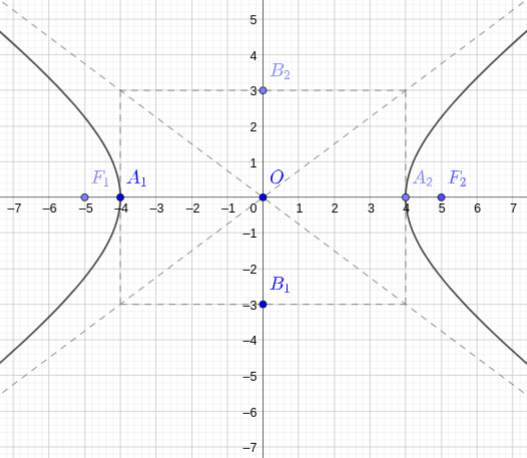
\includegraphics[width=0.7\textwidth]{cap_conicas/dados/fig_ex_hiperbole/fig}
    \caption{Esboço do gráfico da hipérbole de equação $\displaystyle\frac{x^2}{16}-\frac{y^2}{9}=1$.}
    \label{fig:ex_hiperbole}
  \end{figure}  
\end{ex}

\subsection*{Exercícios resolvidos}

\begin{exeresol}
  Obtenha a equação reduzida da hipérbole centrada na origem e de eixo real $|A_1A_2|=8$ e eixo imaginário $|B_1B_2|=4$.
\end{exeresol}
\begin{resol}
  A equação reduzida de uma hipérbole centrada na origem tem a forma
  \begin{equation}
    \frac{x^2}{a^2} - \frac{y^2}{b^2} = 1,
  \end{equation}
  onde $2a = |A_1A_2|$ e $2b=|B_1B_2|$. No caso deste exercício, temos
  \begin{equation}
    2a = 8 \Rightarrow a = 4
  \end{equation}
  e
  \begin{equation}
    2b = 4 \Rightarrow b = 2
  \end{equation}
  Logo, a equação buscada é
  \begin{equation}
    \frac{x^2}{4^2} - \frac{y^2}{2^2} = 1
  \end{equation}
  ou, equivalentemente,
  \begin{equation}
    \frac{x^2}{16} - \frac{y^2}{4} = 1.
  \end{equation}  
\end{resol}

\begin{exeresol}
  Faça o esboço da hipérbole de equação reduzida
  \begin{equation}
    \frac{y^2}{16} - \frac{x^2}{9} = 1.
  \end{equation}
\end{exeresol}
\begin{resol}
  Observe que nesta equação, o termo contendo $x$ tem sinal negativo e o termo contendo $y$ tem sinal positivo (compare com \eqref{eq:hiperbole_red}). Isto nos indica que o eixo real desta hipérbole está na direção das ordenadas $Oy$ e, consequentemente, o eixo imaginário na direção das abscissas $Ox$.

  Da equação, temos $a^2 = 9$ e $b^2=16$, donde $a=3$ e $b=4$. Neste caso, os vértices que definem o eixo real são $A_1=(0, -b)=(0, -4)$ e $A_2=(0, b)=(0, 4)$. Os focos $F_1=(0, -c)$ e $F_2=(0, c)$ são tais que
  \begin{align}
    c^2 &= a^2 + b^2 \\
        &= 9 + 16 \\a
        &= 25 \\
    c &= 5.
  \end{align}
  Com estas informações, traçamos o esboço dado na Figura \ref{fig:hiperbole_exeresol_oy}.

  \begin{figure}[H]
    \centering
    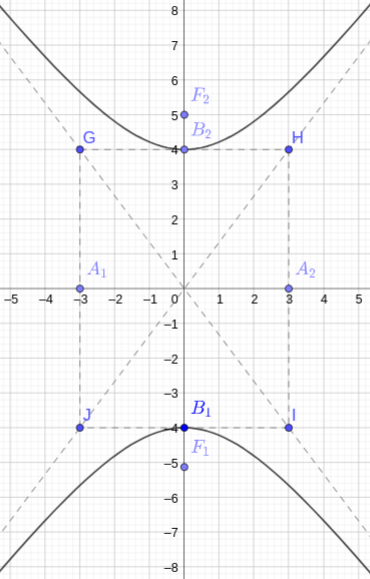
\includegraphics[width=0.5\textwidth]{cap_conicas/dados/fig_hiperbole_exeresol_oy/fig}
    \caption{Esboço do gráfico da hipérbole de equação $\displaystyle\frac{y^2}{16}-\frac{x^2}{9}=1$.}
    \label{fig:hiperbole_exeresol_oy}
  \end{figure}   
\end{resol}

\begin{exeresol}
  Mostre que uma hipérbole de equação reduzida
  \begin{equation}
    \frac{x^2}{a^2} - \frac{y^2}{b^2} = 1
  \end{equation}
  tem assíntotas
  \begin{equation}
    y = \pm \frac{b}{a}x.
  \end{equation}
\end{exeresol}
\begin{resol}
  De fato, ao isolarmos $y$ na equação reduzida, obtemos
  \begin{equation}
    y = \pm\sqrt{\frac{b^2}{a^2}x^2 - b^2}
  \end{equation}
  Logo, para $x\to \infty$, temos
  \begin{gather}
    y\to \pm\sqrt{\frac{b^2}{a^2}x^2} \\
    y\to \pm\sqrt{\frac{b^2}{a^2}}\sqrt{x^2}\\
    y\to \pm\frac{b}{a}x
  \end{gather}
  De forma análoga, quando $x\to -\infty$, temos
  \begin{gather}
    y\to \pm\sqrt{\frac{b^2}{a^2}x^2} \\
    y\to \pm\sqrt{\frac{b^2}{a^2}}\sqrt{x^2}\\
    y\to \mp\frac{b}{a}x
  \end{gather}
  Ambos os resultados mostram que $\displaystyle y=\pm\frac{b}{a}x$ são assíntotas da hipérbole.
\end{resol}

\subsection*{Exercícios}

\begin{exeresol}
  Faça o esboço da hipérbole de equação reduzida
  \begin{equation}
    \frac{x^2}{9} - \frac{y^2}{4} = 1
  \end{equation}
\end{exeresol}
\begin{resp}
  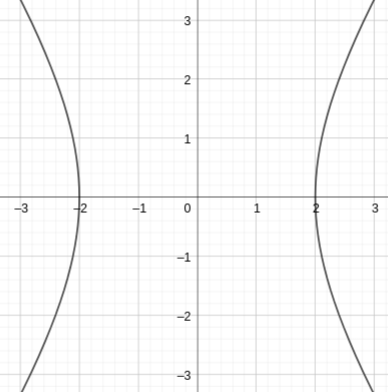
\includegraphics[width=0.5\textwidth]{cap_conicas/dados/fig_hiperbole_exer_ox/fig}
\end{resp}

\begin{exeresol}
  Faça o esboço da hipérbole de equação reduzida
  \begin{equation}
    \frac{y^2}{9} - \frac{x^2}{4} = 1
  \end{equation}
\end{exeresol}
\begin{resp}
  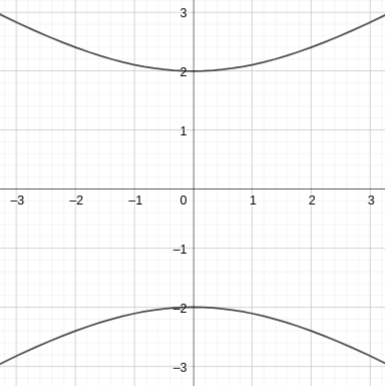
\includegraphics[width=0.5\textwidth]{cap_conicas/dados/fig_hiperbole_exer_oy/fig}
\end{resp}

\begin{exer}
  Determine os vértices do eixo real das seguintes hipérboles:
  \begin{enumerate}[a)]
  \item $\displaystyle \frac{x^2}{9} - \frac{y^2}{4} = 1$
  \item $\displaystyle y^2 - \frac{x^2}{16} = 1$
  \end{enumerate}
\end{exer}
\begin{resp}
  a)~$A_1=(-3,0)$, $A_2=(3,0)$; b)~$B_1=(0, -1)$, $B_2=(0, 1)$
\end{resp}

\begin{exer}
  Determine os focos das seguintes hipérboles:
  \begin{enumerate}[a)]
  \item $\displaystyle \frac{x^2}{9} - \frac{y^2}{4} = 1$
  \item $\displaystyle y^2 - \frac{x^2}{16} = 1$
  \end{enumerate}
\end{exer}
\begin{resp}
  a)~$F_1=(-\sqrt{13}, 0)$, $F_2=(\sqrt{13}, 0)$; b)~$F_1=(0, -\sqrt{17})$, $F_2=(0, \sqrt{17})$
\end{resp}

\begin{exer}
  Forneça a equação reduzida da hipérbole de focos $F_1=(-2, 0)$, $F_2=(2, 0)$ e de vértices do eixo real $A_1=(-1, 0)$ e $A_2=(1, 0)$.
\end{exer}
\begin{resp}
  $\displaystyle x^2 - \frac{y^2}{3} = 1$
\end{resp}

\begin{exer}
  Forneça a equação reduzida da hipérbole de distância focal $|F_1F_2|=2\sqrt{6}$ e de vértices do eixo imaginário $A_1=(-2, 0)$ e $A_2=(2, 0)$.
\end{exer}
\begin{resp}
  $\displaystyle \frac{y^2}{2} - \frac{x^2}{4} = 1$
\end{resp}

\section{Parábola}\label{cap_conicas_sec_parabola}

Em um plano, consideramos uma reta $d$ e um ponto $F$ não pertencente a $d$. Chamamos de \emph{parábola} o conjunto de pontos $P$ do plano que são equidistantes de $F$ e de $d$, i.e.
\begin{equation}
  {\color{blue}\dist(P, F) = \dist(P, d)}.
\end{equation}
Veja a Figura \ref{fig:parabola}.

\begin{figure}[H]
  \centering
  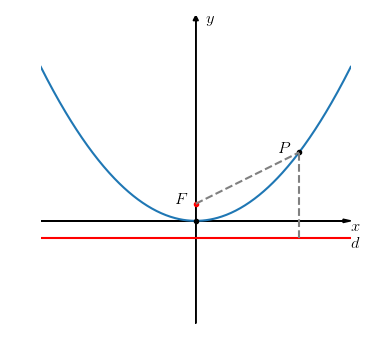
\includegraphics[width=0.7\textwidth]{./cap_conicas/dados/fig_parabola/fig_parabola}
  \caption{Ilustração de uma parábola.}
  \label{fig:parabola}
\end{figure}

O ponto $F$ é chamado de \emph{foco} da parábola. A reta $d$ é chamada de \emph{diretriz} da parábola. A reta perpendicular a $d$ e que passa pelo ponto $F$ é chamada de \emph{eixo} da parábola. O ponto $V$ de interseção entre a parábola e seu eixo é chamado de \emph{vértice} da parábola.

\subsection{Equação reduzida de uma parábola}

Tomamos o sistema cartesiano de coordenadas com origem no vértice da parábola e eixo das abscissas paralelo à diretriz. Seja $p$ tal que
\begin{equation}
  F = (0, p/2).
\end{equation}
Logo, a diretriz tem equação $y = -p/2$. Da definição de parábola, $P=(x,y)$ pertence a parábola quando
\begin{equation}
  \dist(P, F) = \dist(P, d).
\end{equation}
Segue que
\begin{equation}
  \sqrt{x^2+\left(y-\frac{p}{2}\right)^2} = y+\frac{p}{2}.
\end{equation}
Elevando ao quadrado e expandindo, obtemos
\begin{equation}
  x^2 + y^2-py+\frac{p^2}{4} = y^2 + py + \frac{p^2}{4}.
\end{equation}
Cancelando e rearranjando termos, obtemos
\begin{equation}
  {\color{blue}x^2 = 2py},
\end{equation}
a chamada \emph{equação reduzida da parábola}.

\begin{ex}
  A Figura \ref{fig:parabola_ex} é um esboço do gráfica da parábola de equação reduzida
  \begin{equation}
    x^2 = 4y.
  \end{equation}

  \begin{figure}[H]
    \centering
    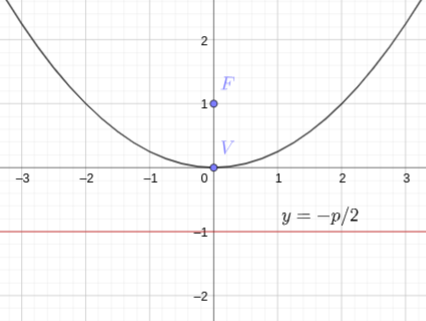
\includegraphics[width=0.6\textwidth]{cap_conicas/dados/fig_parabola_ex/fig}
    \caption{Esboço do gráfico da parábola de equação $y^2 = 4x$.}
    \label{fig:parabola_ex}
  \end{figure}
\end{ex}

\begin{obs}
  Uma parábola com vértice na origem do sistema cartesiano e foco $F=(p/2, 0)$, tem equação reduzida
  \begin{equation}
    y^2 = 2px.
  \end{equation}
\end{obs}

\subsection*{Exercícios resolvidos}

\begin{exeresol}
  Determine a equação reduzida da parábola de diretriz $y=2$ e vértice na origem do sistema cartesiano. Por fim, faça o esboço de seu gráfico.
\end{exeresol}
\begin{resol}
  Uma parábola de equação reduzida
  \begin{equation}
    x^2 = 2py
  \end{equation}
  tem diretriz $\displaystyle y=-\frac{p}{2}$. Logo, sabendo que a diretriz é $y=2$, temos $p = -4$. Então, concluímos que a equação reduzida da parábola é
  \begin{equation}
    x^2 = -8y
  \end{equation}
  A Figura \ref{fig:parabola_exeresol_yp} é o esboço do gráfico desta parábola.

  \begin{figure}[H]
    \centering
    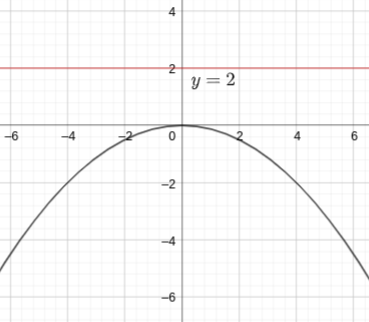
\includegraphics[width=0.6\textwidth]{cap_conicas/dados/fig_parabola_exeresol_yp/fig}
    \caption{Esboço do gráfico da parábola de equação $y^2 = -8x$.}
    \label{fig:parabola_exeresol_yp}
  \end{figure}  
\end{resol}

\begin{exeresol}
  Determine a equação reduzida da parábola de diretriz $x=2$ e vértice na origem do sistema cartesiano. Por fim, faça o esboço de seu gráfico.
\end{exeresol}
\begin{resol}
  Uma parábola de equação reduzida
  \begin{equation}
    y^2 = 2px
  \end{equation}
  tem diretriz $\displaystyle x=-\frac{p}{2}$. Logo, sabendo que a diretriz é $x=2$, temos $p = -4$. Então, concluímos que a equação reduzida da parábola é
  \begin{equation}
    y^2 = -8x
  \end{equation}
  A Figura \ref{fig:parabola_exeresol_xp} é o esboço do gráfico desta parábola.

  \begin{figure}[H]
    \centering
    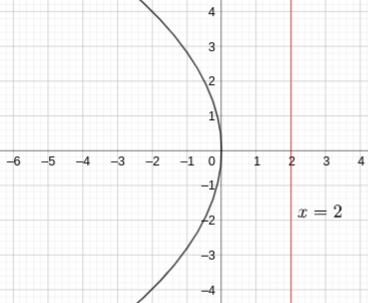
\includegraphics[width=0.6\textwidth]{cap_conicas/dados/fig_parabola_exeresol_xp/fig}
    \caption{Esboço do gráfico da parábola de equação $y^2 = -8x$.}
    \label{fig:parabola_exeresol_xp}
  \end{figure}  
\end{resol}

\subsection*{Exercícios}

\begin{exer}
  Faça o esboço do gráfico da parábola de equação reduzida
  \begin{equation}
    x^2 = 2y.
  \end{equation}
  Identifique no esboço a reta diretriz, o foco e o vértice da parábola.
\end{exer}
\begin{resp}
  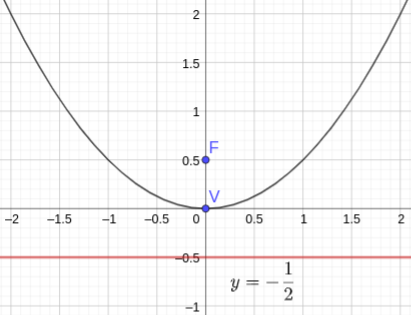
\includegraphics[width=0.5\textwidth]{cap_conicas/dados/fig_parabola_exer_x2_2y/fig}
\end{resp}

\begin{exer}
  Faça o esboço do gráfico da parábola de equação reduzida
  \begin{equation}
    x^2 = -2y.
  \end{equation}
  Identifique no esboço a reta diretriz, o foco e o vértice da parábola.
\end{exer}
\begin{resp}
  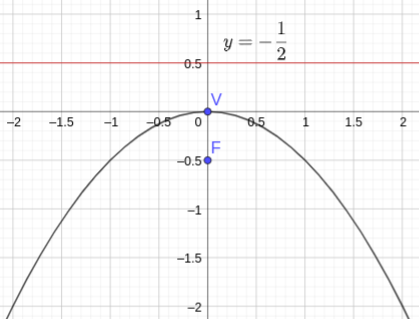
\includegraphics[width=0.5\textwidth]{cap_conicas/dados/fig_parabola_exer_x2-2y/fig}
\end{resp}

\begin{exer}
  Faça o esboço do gráfico da parábola de equação reduzida
  \begin{equation}
    y^2 = 2x.
  \end{equation}
  Identifique no esboço a reta diretriz, o foco e o vértice da parábola.
\end{exer}
\begin{resp}
  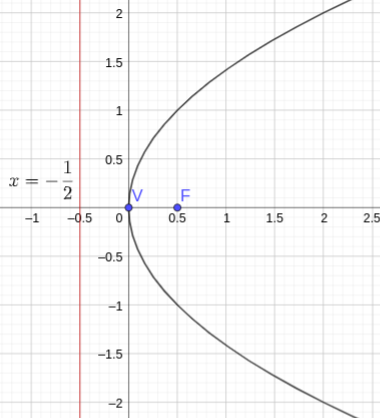
\includegraphics[width=0.5\textwidth]{cap_conicas/dados/fig_parabola_exer_y2_2x/fig}
\end{resp}

\begin{exer}
  Faça o esboço do gráfico da parábola de equação reduzida
  \begin{equation}
    y^2 = -2x.
  \end{equation}
  Identifique no esboço a reta diretriz, o foco e o vértice da parábola.
\end{exer}
\begin{resp}
  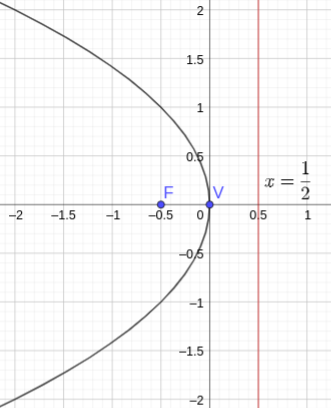
\includegraphics[width=0.5\textwidth]{cap_conicas/dados/fig_parabola_exer_y2-2x/fig}
\end{resp}

\begin{exer}
  Determine o foco de cada uma das seguintes parábolas:
  \begin{enumerate}[a)]
  \item $y = 2x^2$
  \item $y + 2x^2 = 0$
  \item $y^2 + 4x = 0$
  \item $\frac{1}{4}y^2 = x$
  \end{enumerate}
\end{exer}
\begin{resp}
  a)~$F=(0, \frac{1}{8})$; b)~$F=(0, -\frac{1}{8})$; c)~$F=(-1, 0)$; d)~$F=(1, 0)$
\end{resp}
